\chapter{基本语法}
\label{chap:grammar}


\section{基本规范}

\textbf{Java区分大小写}

Java采用骆驼命名法,CamelCase。

\section{数据类型}

Java包含8种基本类型。\par
\begin{itemize}
        \item   4种整型
        \item   2种浮点类型 
        \item   1种表示Unicode编码的字符单元的字符类型char
        \item   1种表示真值的boolean类型
\end{itemize}


\subsection{整型}

\renewcommand\arraystretch{2}
\begin{tabular}{l|l|l}
    类型        &      存储需求        &     取值范围        \\               \hline
    byte       &       1字节          & -128 $\sim$ 127     \\
    short      &       2字节          & -32768 $\sim$ 32767  \\
    int        &       4字节          &  -2147483648 $\sim$ 2147483647  \\
    long       &       8字节          &  -9223372036854775808 $\sim$ 9223372036854775807  \\
\end{tabular}\newline

\notebox{Java 没有任何无符号(unsigned)形式的整型。}

长整型值有一个后缀l或者L。

\begin{lstlisting}[style=cjava]
        long number = 123L;             // number值为:123
\end{lstlisting}


\begin{itemize}
    \item   二进制带前缀0b或者0B (从java 7开始)
    \item   八进制带前缀0
    \item   十六进制带前缀0x或者0X
\end{itemize}


\begin{lstlisting}[style=cjava]
        int binaryNumber      = 0B101;              // 二进制表示   5 

        int hexadecimalNumber = 0x123;              // 十六进制表示 291   

        int octonaryNumber    = 0123;              // 八进制表示   83
\end{lstlisting}



同样从Java7开始为数字加下划线,Java编译器会去除这些下划线

\begin{lstlisting}[language=java]
        Sytem.out.println(0_1_0);       // 010表示八进制,输出8
\end{lstlisting}


\subsubsection{整数类型操作}

\begin{itemize}
        \item   toBinaryString  将整数转为二进制位字符串
        \item   bitCount        计算整数bit位为 1的个数
        \item   ...
    \end{itemize}

\begin{lstlisting}[language=java]
        System.out.println(Integer.toBinaryString(666));
        System.out.println(Integer.toBinaryString(-1));
        System.out.println(Integer.bitCount(0B10_10011010));

        /**
         * 1010011010
         * 11111111111111111111111111111111
         * 5
         */
\end{lstlisting}
    


\cautionbox{
注意JS INT类型的值范围:
\begin{itemize}
        \item   \href{http://speakingjs.com/es5/ch11.html}{Integers in JavaScript} 
        \item   \href{http://speakingjs.com/es5/ch11.html\#safe\_integers}{Safe Integers}
        \end{itemize}
}


\subsection{浮点数}


\renewcommand\arraystretch{2}
\begin{tabular}{l|l|l}
    类型         &      存储需求        &     取值范围        \\               \hline
    float        &       4字节          & 有效位数为6-7位      \\
    double      &       8字节          & 有效位数为15位       \\
\end{tabular}\newline


float类型的值要有后缀f或者F。没有后缀默认为double类型。

double类型也可以添加d或者D后缀。


用于表示溢出或者出错情况的三个特殊浮点值:

\begin{itemize}
        \item   正无穷大  
        \item   负无穷大
        \item   NaN (不是一个数字)
\end{itemize}

例如: 一个正整数除以 0 的结果为正无穷大; 计算 0/0或者负数的平方根结果为NaN。

对应常量为:
\begin{lstlisting}[language=java]
        // float
        Float.POSITIVE_INFINITY;
        Float.NEGATIVE_INFINITY;
        Float.NaN;
        // double
        Double.POSITIVE_INFINITY;
        Double.NEGATIVE_INFINITY;
        Double.NaN;
\end{lstlisting}


所有“非数值”的值都认为是不相同的。

\begin{lstlisting}[language=java]
        if(Double.isNaN(x))   // check whether x is "not a number"
\end{lstlisting}




\textbf{char类型}


\section{运算符}

\subsection{位运算符}

\renewcommand\arraystretch{2}
\begin{tabular}{l|l|l}
    操作符    &     名称          &     说明                                                       \\   \hline
    \~{}     &  Not(按位取反)   & 一元运算符   \quad 0变为1、将1变为0                                \\
    \&       &   And(按位与)    & 二元运算符   \quad 两值全为1则为1 \quad 例:1\&1=1                 \\
    |       &   Or(按位或)     & 二元运算符    \quad 两值有1则为1 \quad 例: 0|1=1                   \\
    \^{}     &   Xor(按位异或)  & 二元运算符    \quad 两值不相同则异或结果为1 \quad 例: 1\^{}0=1       \\
    <<       &  左移位           & 二元运算符    \quad                                               \\
    >>       &  右移位           & 二元运算符    \quad 符号运算符会填充高位                             \\ 
    >>>      & 无符号右移位       & 二元运算符    \quad 运算符会用0填充高位                              \\
\end{tabular}\newline


\subsubsection{移位}

\begin{lstlisting}[language=java]
        /**
        * 下一个2的幂;普通性能
        *
        * @param numElements
        * @return
        */
       public static int calculateSize(int numElements) {
           int initialCapacity = 8;
           while (initialCapacity < numElements) initialCapacity <<= 1;
           return initialCapacity;
       }
   
   
       /*
        * ArrayDeque 扩容原理;下一个2的幂;比上面的函数性能更好
        */
       private static int calculateSize(int numElements) {
           int initialCapacity = 8;
           // Find the best power of two to hold elements.
           // Tests "<=" because arrays aren't kept full.
           if (numElements >= initialCapacity) {
               initialCapacity = numElements;
               initialCapacity |= (initialCapacity >>> 1);
               initialCapacity |= (initialCapacity >>> 2);
               initialCapacity |= (initialCapacity >>> 4);
               initialCapacity |= (initialCapacity >>> 8);
               initialCapacity |= (initialCapacity >>> 16);
               initialCapacity++;
   
               if (initialCapacity < 0)   // Too many elements, must back off
                   initialCapacity >>>= 1;// Good luck allocating 2 ^ 30 elements
           }
           return initialCapacity;
       }
   
\end{lstlisting}


\subsubsection{与操作符}

判断某个正数字是否为2的幂次方

如果 N 与 N -1 相与则此数为2的幂次方

\begin{lstlisting}[language=java]
        /**
        * 判断非零正整数是否为2的幂次方
        * @param number
        * @return
        */
       public boolean isPowerOfTwo(int number) {
           if (number <= 0) {
               return false;
           }
   
           return (number & (number - 1)) == 0;
       }

\end{lstlisting}


字节顺序


对于w位的操作数$x$用位表示为 [$x_{w-1}$, $x_{w-2}$, ... , $x_{0}$, $x_{0}$ ]。
其中$x_{w-1}$是最高有效位,而$x_{0}$是最低有效位。

小端法(little endian): 选择在内存中按照从最低有效字节到最高有效字节的顺序存储对象

大端法(big endian): 选择在内存中按照从最高有效字节到最低字节的顺序存储对象

假设变量x的类型为int,位于地址0x100处,它的十六进制值为0x1234567。地址范围0x100 ~ 0x103的字节顺序。


\begin{figure}[H]
        \centering
        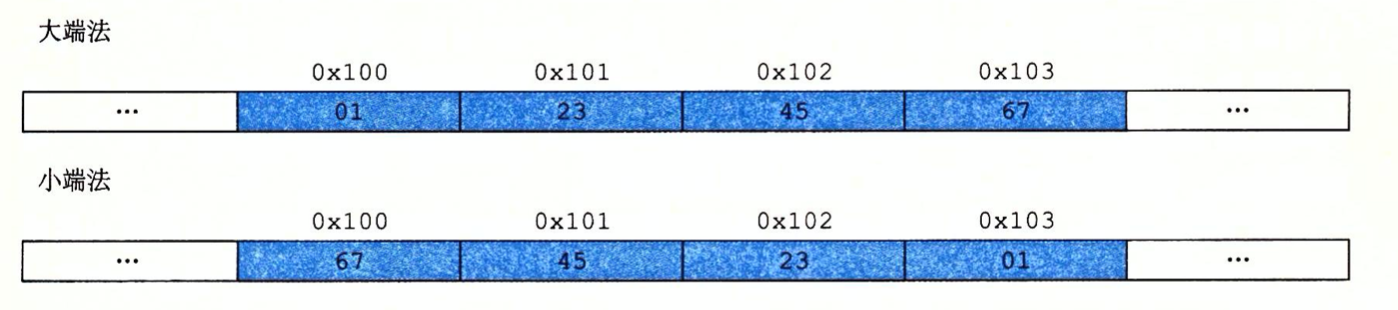
\includegraphics[width=1\textwidth]{basic/big_little_endian.png}
    \end{figure}


移位运算符的右操作数会先完成取模运算。int类型模32,long类型模64。


\begin{lstlisting}[language=java]

\end{lstlisting}




避免时序攻击的字符串比较

\begin{lstlisting}[language=java]

        static boolean equals(byte[] s1, byte[] s2) {
                if (s1.length != s2.length) {
                  return false;
                }
                char c = 0;
                for (int i = 0; i < s1.length; i++) {
                  c |= (s1[i] ^ s2[i]);
                }
                return c == 0;
              }
        
\end{lstlisting}













































